\documentclass[10pt]{article} 
\usepackage{amsmath}
\usepackage{cancel}
\usepackage{geometry}
\usepackage{graphicx}
\graphicspath{ {./images/} }
\geometry{legalpaper, margin=1.25in}
\usepackage[parfill]{parskip}

\setlength{\parindent}{0pt}



\title{Notes on Fourier Stability Analysis}
\author{Tristan Ball}


\begin{document}

\maketitle
\tableofcontents
\pagebreak


\section{Introduction to Fourier Analysis}

	One way to analyze the stability of a scheme is to take the Fourier Transform of the continuous PDE and compare to the Fourier Transform of the discrete scheme. Since the Fourier Transform will yield a system of decoupled ODE's, we can compare the eigenvalues of the analytical and numerical versions.  
	
	The wave number is defined as follows:

	\begin{equation}
		k = \frac{2 \pi}{\lambda} = \frac{2 \pi n}{L}, \; n \epsilon [1,\infty]
	\end{equation}

	The wavelength ($\lambda$) must be at least as large as two grid cells (with a width of $\Delta x$) in order to fully capture the wave in the mesh. Therefore, the wave number must lie in the following range:

	\begin{equation}
		\begin{aligned}
			0 \leq k \leq \frac{2 \pi}{2 \Delta x} \\
			0 \leq k \Delta x \leq \pi 
		\end{aligned}
	\end{equation}


\section{Fourier Analysis of Semi-Discrete 1D Heat Equation}

	Consider the one dimensional heat equation,
	
	\begin{equation} \label{1D_heat}
		\frac{\partial u}{\partial t} - \nu \frac{\partial^2 u}{\partial x^2} = 0
	\end{equation}

	Take the Fourier Transform of (\ref{1D_heat}):
	
	\begin{equation} \label{1D_heat_FT}
		\frac{1}{\sqrt{2}\pi} \int_{-\infty}^{\infty} \left( \frac{\partial u}{\partial t} - \nu \frac{\partial^2 u}{\partial x^2} \right) e^{-ikx} dx = 0
	\end{equation}

	Simplify (\ref{1D_heat_FT}):
	
	\begin{equation} \label{1D_heat_FT2}
		\frac{\partial}{\partial t} \left[ \frac{1}{\sqrt{2}\pi} \int_{-\infty}^{\infty} u e^{-ikx} dx \right] - \frac{\nu}{\sqrt{2}\pi} \int_{-\infty}^{\infty} \frac{\partial^2 u}{\partial x^2}  e^{-ikx} dx = 0
	\end{equation}

	The first term in (\ref{1D_heat_FT2}) contains the definition of the Fourier Transform, $\tilde{u}$, and the second term needs to be simplified further. Applying integration by parts to the integral in the second term, we get

	\begin{equation} \label{1D_heat_FT3}
		\frac{\partial u}{\partial x} e^{-ikx} \Big|_{-\infty}^{\infty} - \int_{-\infty}^{\infty} \frac{\partial u}{\partial x} (-ik) e^{-ikx} dx
	\end{equation}
	
	The first term of (\ref{1D_heat_FT3}) goes to zero as x approaches infinity. We can apply integration by parts again to simplify this integral.
	
	\begin{equation} \label{1D_heat_FT4}
		iku e^{-ikx} \Big|_{-\infty}^{\infty} + \int_{-\infty}^{\infty} u (-ik)^2 e^{-ikx} dx
	\end{equation}

	Again, the first term of (\ref{1D_heat_FT4}) goes to zero as x approaches infinity. Now, (\ref{1D_heat_FT4}) simplifies to
	
	\begin{equation} \label{1D_heat_FT5}
		(-ik)^2 \int_{-\infty}^{\infty} u e^{-ikx} dx = (-ik)^2 \tilde{u}
	\end{equation}

	Putting (\ref{1D_heat_FT5}) back into equation (\ref{1D_heat_FT2}), we get the final form for the PDE:
	
	\begin{equation} \label{1D_heat_FT6}
		\begin{aligned}
			\frac{\partial \tilde{u}}{\partial t} - \nu (-ik)^2 \tilde{u} = 0 \\
			\frac{\partial \tilde{u}}{\partial t} + \nu k^2 \tilde{u} = 0
		\end{aligned}
	\end{equation}

	

	Now Fourier Transform a semi-discrete approximation of (\ref{1D_heat}) using a central differencing scheme in space:
	
	\begin{equation} \label{1D_heat_semi}
		\begin{aligned}
			\frac{du_i}{dt} &= \nu \frac{u_{i+1} - 2u_i + u_{i-1}}{\Delta x^2}\\
			\frac{d \tilde u}{dt} &= \frac{\nu}{\Delta x^2} \left( e^{ik \Delta x} - 2 + e^{-ik \Delta x} \right) \tilde{u} \\
			\frac{d \tilde u}{dt} &= - \frac{\nu}{\Delta x^2} \left( 2 - 2cos(k \Delta x) \right) \tilde{u} \\
			\frac{d \tilde u}{dt} &= - \frac{2 \nu}{\Delta x^2} \left( 1 - cos(k \Delta x) \right) \tilde{u}
		\end{aligned}
	\end{equation}

	We can compare the analytical solution with the numerical solution, i.e. the Fourier Transformed PDE with the semi-discrete equation. We can write equation (\ref{1D_heat_FT6}) in the following way to make the comparison easier:
	
	\begin{equation} \label{1D_heat_FT7}
		\frac{d \tilde u}{dt} = -\frac{\nu}{\Delta x^2} (k \Delta x)^2 \tilde{u}
	\end{equation}

	Plotting the eigenvalues of the numerical scheme vs the analytical equation, we can analyze the stability.
	
	\begin{figure}[h]
		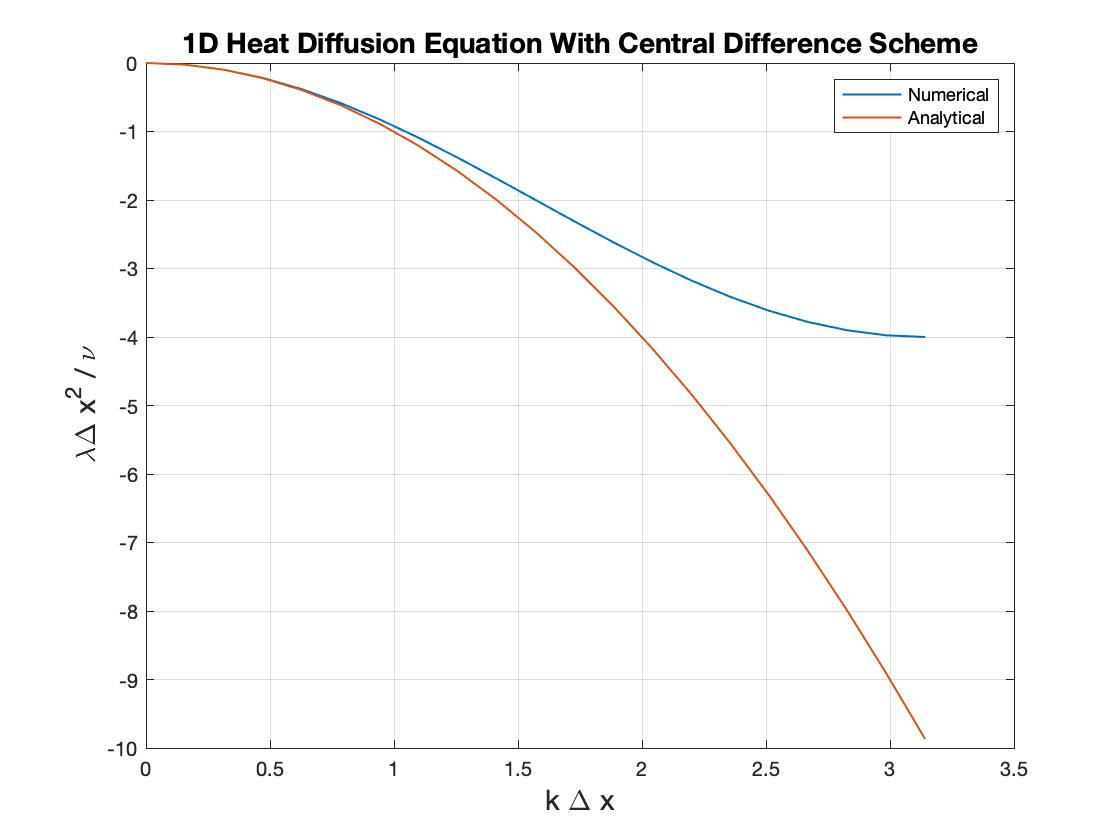
\includegraphics[width=12cm]{heat_central}
		\centering
	\end{figure}
	
	From this figure, it can be seen that the numerical approximation will be more accurate for smaller values of $k \Delta x$.
	
	Note that both the PDE and central difference discretization in space yielded only real eigenvalues. This will generate a symmetric matrix.
	
\section{Fourier Analysis of Semi-Discrete 1D Wave Equation}
	
	Consider the one dimensional wave equation,
	
	\begin{equation} \label{1D_wave}
		\frac{\partial u}{\partial t} + a \frac{\partial u}{\partial x} = 0
	\end{equation}
	
	Take the Fourier Transform of (\ref{1D_wave}):
	
	\begin{equation} \label{1D_wave_FT}
		\frac{1}{\sqrt{2}\pi} \int_{-\infty}^{\infty} \left( \frac{\partial u}{\partial t} + a \frac{\partial u}{\partial x} \right) e^{-ikx} dx = 0
	\end{equation}
	
	Simplify (\ref{1D_wave_FT}):
	
	\begin{equation} \label{1D_wave_FT2}
		\frac{\partial}{\partial t} \left[ \frac{1}{\sqrt{2}\pi} \int_{-\infty}^{\infty} u e^{-ikx} dx \right] + \frac{a}{\sqrt{2}\pi} \int_{-\infty}^{\infty} \frac{\partial u}{\partial x}  e^{-ikx} dx = 0
	\end{equation}
	
	The first term in (\ref{1D_wave_FT2}) contains the definition of the Fourier Transform, $\tilde{u}$, and the second term needs to be simplified further. Applying integration by parts to the integral in the second term, we get
	
	\begin{equation} \label{1D_wave_FT3}
		u e^{-ikx} \Big|_{-\infty}^{\infty} - \int_{-\infty}^{\infty} u (-ik) e^{-ikx} dx
	\end{equation}
	
	Assuming that $u$ goes to zero as $x$ approaches infinity, the first term of (\ref{1D_wave_FT3}) goes to zero. Now, (\ref{1D_wave_FT3}) simplifies to
	
	\begin{equation} \label{1D_wave_FT4}
		(-ik)^2 \int_{-\infty}^{\infty} u e^{-ikx} dx
	\end{equation}
	
	Putting (\ref{1D_wave_FT4}) back into equation (\ref{1D_wave_FT2}), we get
	
	\begin{equation} \label{1D_wave_FT5}
			\frac{\partial \tilde{u}}{\partial t} +aik \tilde{u} = 0
	\end{equation}
	
	Now apply the Fourier Transform to a semi-discrete approximation of (\ref{1D_wave}) using a central differencing scheme in space:
	
	\begin{equation} \label{1D_wave_semi}
		\begin{aligned}
			\frac{du_i}{dt} &= - a \frac{u_{i+1} - u_{i-1}}{2 \Delta x} \\
			\frac{d \tilde u}{dt} &= - \frac{a}{\Delta x} \left( \frac{e^{ik \Delta x} - e^{-ik \Delta x}}{2} \right) \tilde{u} \\
			\frac{d \tilde u}{dt} &= -i \frac{a}{\Delta x} sin(k \Delta x) \tilde{u}
		\end{aligned}
	\end{equation}
	
	We can compare the analytical solution with the numerical solution, i.e. the Fourier Transformed PDE with the semi-discrete PDE. We can write equation (\ref{1D_wave_FT5}) in the following way to make the comparison easier:
	
	\begin{equation} \label{1D_wave_FT6}
		\frac{d \tilde u}{dt} = -i \frac{a}{\Delta x} k \Delta x \tilde{u}
	\end{equation}
	
	Plotting the central difference scheme vs the analytical equation, we can analyze the stability.
	
	\begin{figure}[h]
		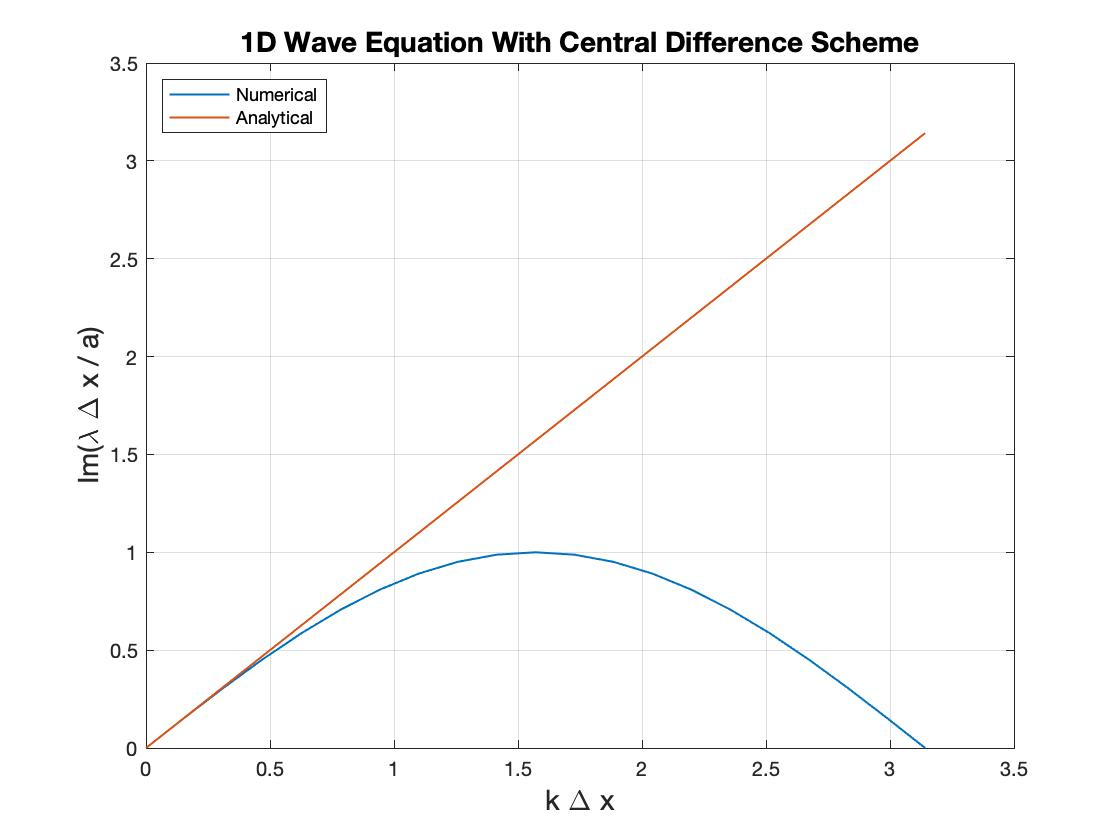
\includegraphics[width=12cm]{wave_central}
		\centering
	\end{figure}

	From this figure, we can see that at high wave numbers, we will experience odd-even decoupling since the analytical solution goes back to zero as the numerical solution rises to $\pi$. This will result in the approximation blowing up since energies from adjacent spacial grid points in the discretization will not go anywhere.
	
	Now we will apply an upwind scheme and compare with the central difference scheme and analytical solution.
	
	\begin{equation} \label{1D_wave_semi2}
		\begin{aligned}
			\frac{du_i}{dt} &= - a \frac{u_{i} - u_{i-1}}{\Delta x} \\
			\frac{d \tilde u}{dt} &= - \frac{a}{\Delta x} \left( \tilde{u} - e^{-ik \Delta x} \tilde{u} \right) \\
			\frac{d \tilde u}{dt} &= - \frac{a}{\Delta x} \left( 1- e^{-ik \Delta x} \right) \tilde{u} \\
			\frac{d \tilde u}{dt} &= - \frac{a}{\Delta x} \left[ 1 - (cos(k \Delta x) + i sin(k \Delta x)) \right] \tilde{u} 
		\end{aligned}
	\end{equation}
	
	Plotting the upwind scheme vs the analytical equation, we can analyze the stability.
	
	\begin{figure}[h]
		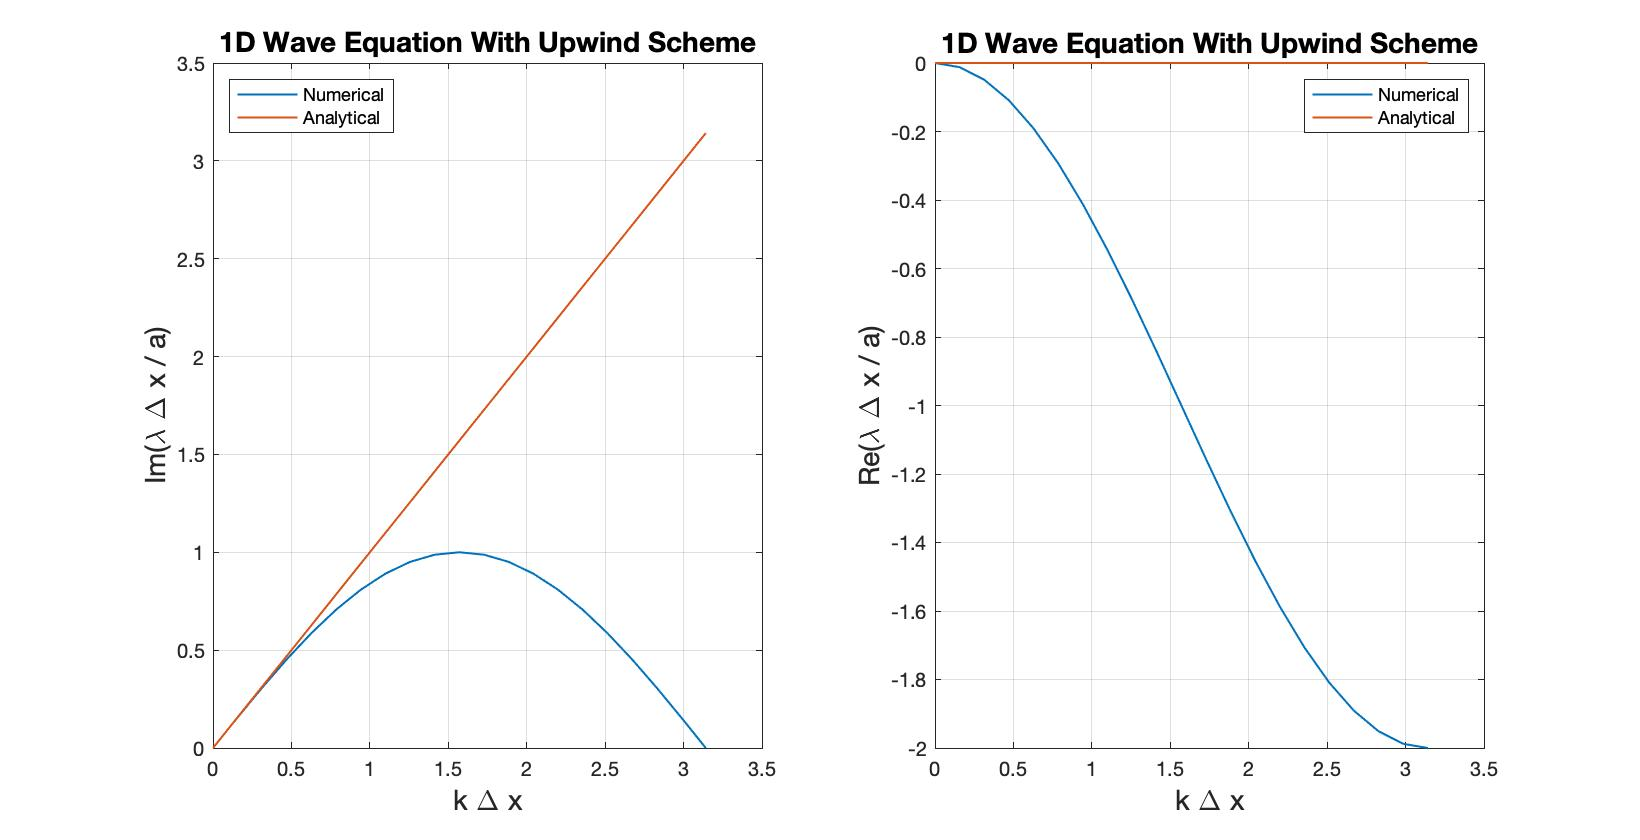
\includegraphics[width=16cm]{wave_upwind}
		\centering
	\end{figure}

	From this figure, we again see odd-even decoupling in the complex plane, however the effect is damped by the real plane. In the real plane, the numerical solution decreases while the analytical solution is constant. This will dissipate the energies not passed on by adjacent steps in the spacial grid and prevent the approximation from blowing up.
	
\section{Fourier Analysis of 1D DGFEM Wave Equation}

	This analysis can be applied to FEM techniques as well, but requires manipulation of circulant matrices. 
	
	For example, a circulant matrix with three entries can be described as follows:
	
	\[
	\begin{bmatrix}
		B & C & \hdots & \hdots & A\\
		A & B & C & \hdots& \hdots\\
		& A & B & C & \hdots\\
		& & \ddots\\
		C & \hdots & \hdots& A & B
	\end{bmatrix}
	\]
	
	The following is a discretization using DG on the 1D wave equation with upwinding. See Notes on DG Formulation for details.
	
	\begin{align}
		{\bf{M}} \frac{du}{dt} \frac{\Delta x}{2} + \hat{f} - {\bf{K}}ua = 0 \\
		\frac{du}{dt} = {\bf{M}}^{-1}[{\bf{K}}ua - \hat{f}]\frac{2}{\Delta x}
	\end{align}

	For P=1, the circulant matrix system reduces to 
	
	\begin{align}
		\frac{du}{dt} = {\bf{M}}^{-1} (B\vec{u}\;^n + A\vec{u}\;^{n-1}) \frac{2a}{\Delta x} \\
		\frac{du}{dt} - {\bf{M}}^{-1} (B + Ae^{-i\theta}) \frac{2a}{\Delta x}\vec{u} = 0
	\end{align}

	\[
	\begin{bmatrix}
		B & A\\
		A & B
	\end{bmatrix}
	\begin{bmatrix}
		\binom{u_0}{u_1}_1\\
		\binom{u_0}{u_1}_2
	\end{bmatrix}
	=0
	\]
	
	Here, 
	\[B = 
	\begin{bmatrix}
		-1/2 & -1/2\\
		1/2 & -1/2
	\end{bmatrix}\]
	\[A = 
	\begin{bmatrix}
		0 & 1\\
		0 & 0
	\end{bmatrix}\]

	As a test case, try a=1 and dx=1/12. The eigenvalues of this system can be calculated using computer software. Plotting these values yields the following:
	
	
	
	
\section{1D Euler Equations}

	For systems of equations, it is easiest to analyze the stability by visually inspecting a plot of the eigenvalues on the real-imaginary plane.

	1D conservation law:

	\begin{equation} \label{1D_euler}
		\frac{\partial \mathbf{w}}{\partial t} + \frac{\partial \mathbf{F}}{\partial x} = 0
	\end{equation}

	$${\mathbf{w}} = \left[
	\begin{tabular}{c}
		$\rho$\ \\
		$\rho u$ \\
		$\rho E$ 
	\end{tabular}
	\right], \quad
	{\mathbf{F}} = \left[
	\begin{tabular}{c}
		$\rho u$ \\
		$\rho u^2+P$ \\
		$\rho u (E + P/\rho)$ 
	\end{tabular}
	\right]
	$$
	
	
	The flux can be rewritten as:
	
	$${\mathbf{F} (\mathbf{w})} = \left[
	\begin{tabular}{c}
		$w_2$\ \\
		$w^2_2/w1 + (\gamma - 1) * (w_3 - 0.5 * w_2^2 / w_1)$ \\
		$w_2 / w_1 * (w_3 + (\gamma - 1)*(w_3 - 0.5 * w_2^2 / w_1))$ 
	\end{tabular}
	\right]
	$$
	
	
	Linearize (\ref{1D_euler}) with chain rule:
	
	\begin{equation} \label{1D_euler_linearized}
		\frac{\partial \mathbf{w}}{\partial t} + \frac{\partial \mathbf{F}}{\partial \mathbf{w}} \frac{\partial \mathbf{w}}{\partial x} = 0
	\end{equation}

	Computing the eigenvalues of the Jacobian $\mathbf{J} = \frac{\partial \mathbf{F}}{\partial \mathbf{w}}$ yields the following:
	
		$$eig(\mathbf{J}) = 
		\begin{bmatrix}
			u & 0 & 0 \\
			0 & u+c & 0 \\
			0 & 0 & u-c
		\end{bmatrix}$$

	The 1D Euler equations are essentially a first order system of three decoupled wave equations with wave speeds $u$, $u+c$ and $u-c$. We can upwind each of these equations using artificial diffusion as follows:
	
	\begin{equation} \label{1D_euler_upwind}
		\frac{\partial \mathbf{w}}{\partial t} = - \left( A \frac{\partial \mathbf{w}}{\partial x} - adis * \frac{|A|}{2} \left( \frac{\partial^2 \mathbf{w}}{\partial x^2} \right) \right)
	\end{equation}

	Where $adis$ is a dissipation constant. Since A is a matrix, $|A|$ must be calculated from the eigenvalue problem as
	
	\begin{equation}
		|A| = V*|E|*V^{-1}
	\end{equation}

	It is convenient to define Fourier operators for the derivatives in the $x$ direction. For the first and second derivatives, we can use:
	
	$$
	\frac{\partial}{\partial x} = \frac{i sin(k \Delta x)}{\Delta x}
	, \quad
	\frac{\partial^2}{\partial x^2} = - \frac{2-2cos(k \Delta x)}{\Delta x^2}
	$$
	
	The eigenvalues of the right hand side of (\ref{1D_euler_upwind}) can be calculated for $-\pi < k < \pi$ using the Fourier operators. Plotting the eigenvalues yields three circles that represent the eigenvalues of the three uncoupled wave equations.
	
	The eigenvalue plot is shown below using a flow state with parameters $\gamma = 1.4$, $P_0 = 1.015\mathrm{e}5$ Pa, $T_0 = 300$ K, $\bar{R} = 8314$ J/kmol $\cdot$ K, $M_w = 28.9$, $adis = 1.0$ and a base flow velocity of $u=0.1*c$. Wavenumbers are shown from $-\pi<k<\pi$ in increments of $\pi/30$.
	
	\begin{figure}[h]
		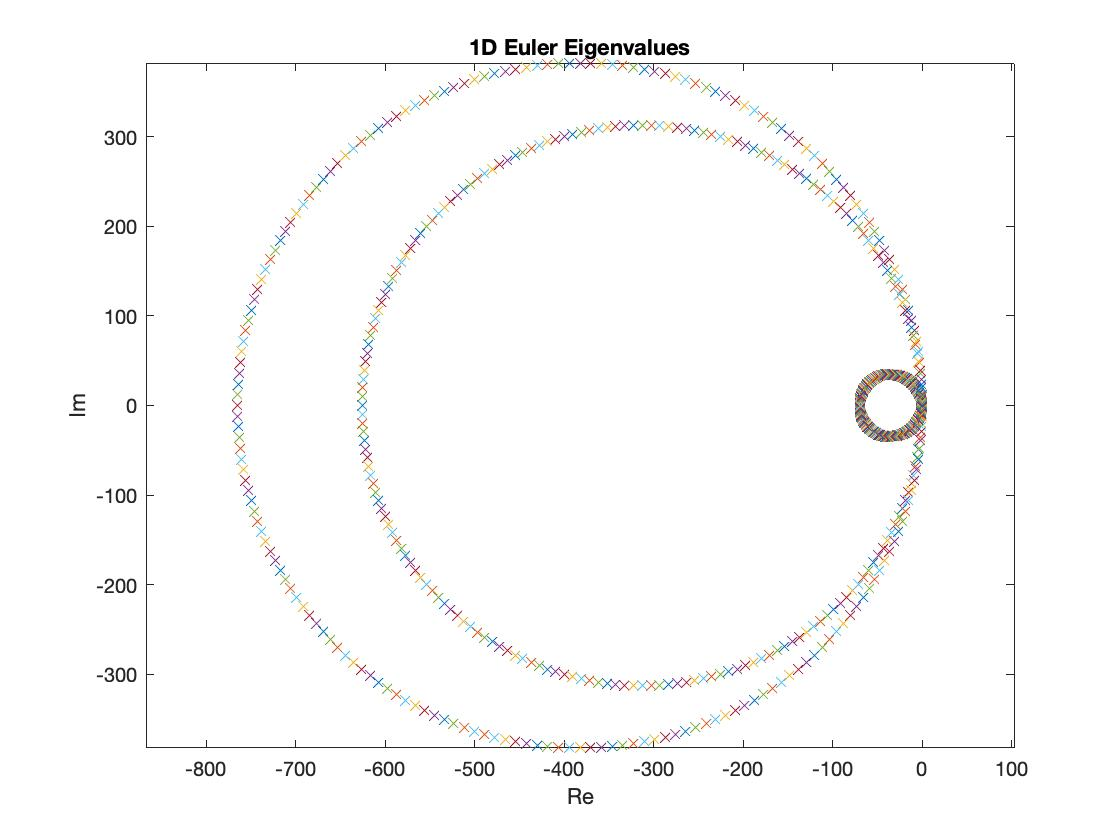
\includegraphics[width=12cm]{1D_euler_eig}
		\centering
	\end{figure}
	
	
\section{2D Euler Equations}

	Again, it is easiest to analyze the stability by visually inspecting a plot of the eigenvalues on the real-imaginary plane.
	
	2D conservation law:

	\begin{equation} \label{2D_euler}
		\frac{\partial \mathbf{w}}{\partial t} + \frac{\partial \mathbf{F_x}}{\partial x} + \frac{\partial \mathbf{F_y}}{\partial y} = 0
	\end{equation}


	$${\mathbf{w}} = \left[
	\begin{tabular}{c}
		$\rho$\ \\
		$\rho u_x$ \\
		$\rho u_y$ \\
		$\rho E$ 
	\end{tabular}
	\right], \quad
	{\mathbf{F_x}} = \left[
	\begin{tabular}{c}
		$\rho u_x$ \\
		$\rho u^2_x+P$ \\
		$\rho u_x u_y$ \\
		$\rho u_x (E + P/\rho)$ 
	\end{tabular}
	\right] ,\quad
	{\mathbf{F_y}} = \left[
	\begin{tabular}{c}
		$\rho u_y$ \\
		$\rho u_x u_y$ \\
		$\rho u^2_y+P$ \\
		$\rho u_y (E + P/\rho)$ 
	\end{tabular}
	\right] ,\quad
	$$
	
	
	The fluxes can be rewritten as:
	
	$${\mathbf{F_x} (\mathbf{w})} = \left[
	\begin{tabular}{c}
		$w_2$\ \\
		$w^2_2/w_1+(\gamma-1)*(w_4-0.5*(w^2_2+w^2_3)/w_1)$ \\
		$ w_2*w_3/w_1$ \\
		$w_2/w_1*(w_4+(\gamma-1)*(w_4-0.5*(w^2_2+w^2_3)/w_1))$ 
	\end{tabular}
	\right]
	$$
	
	$${\mathbf{F_y} (\mathbf{w})} = \left[
	\begin{tabular}{c}
		$w_3$\ \\
		$ w_2*w_3/w_1$ \\
		$w^2_3/w_1+(\gamma-1)*(w_4-0.5*(w^2_2+w^2_3)/w_1)$ \\
		$w_3/w_1*(w_4+(\gamma-1)*(w_4-0.5*(w^2_2+w^2_3)/w_1))$ 
	\end{tabular}
	\right]
	$$
	

	Linearize (\ref{2D_euler}) with chain rule:
	
	\begin{equation} \label{2D_euler_linearized}
		\frac{\partial \mathbf{w}}{\partial t} + \frac{\partial \mathbf{F_x}}{\partial \mathbf{w}} \frac{\partial \mathbf{w}}{\partial x} + \frac{\partial \mathbf{F_y}}{\partial \mathbf{w}} \frac{\partial \mathbf{w}}{\partial y}= 0
	\end{equation}
	
	Computing the eigenvalues of the Jacobians $\mathbf{J_x} = \frac{\partial \mathbf{F_x}}{\partial \mathbf{w}}$ and $\mathbf{J_y} = \frac{\partial \mathbf{F_y}}{\partial \mathbf{w}}$ yields the following:
	
		$$eig(\mathbf{J_x}) = 
		\begin{bmatrix}
			u & 0 & 0 & 0\\
			0 & u & 0 & 0\\
			0 & 0 & u+c & 0 \\
			0 & 0 &0 & u-c
		\end{bmatrix}, \quad
		eig(\mathbf{J_y}) = 
		\begin{bmatrix}
			v & 0 & 0 & 0\\
			0 & v & 0 & 0\\
			0 & 0 & v+c & 0 \\
			0 & 0 &0 & v-c
		\end{bmatrix}$$
	
	Similar to the 1D Euler equations, we can upwind equation (\ref{2D_euler_linearized}) using artificial diffusion as follows:
	
	\begin{equation} \label{2D_euler_upwind}
		\frac{\partial \mathbf{w}}{\partial t} = - \left( A_x \frac{\partial \mathbf{w}}{\partial x} - adis * \frac{|A_x|}{2} \left( \frac{\partial^2 \mathbf{w}}{\partial x^2} \right) \right) - \left( A_y \frac{\partial \mathbf{w}}{\partial y} - adis * \frac{|A_y|}{2} \left( \frac{\partial^2 \mathbf{w}}{\partial y^2} \right) \right)
	\end{equation}
	
	Here, the Fourier operators can be used on the $x$ direction derivatives, however a central difference will be used for the $y$ direction derivatives. This will result in a block tri-diagonal matrix for which the eigenvalues can be calculated and plotted. For this case, periodic boundary conditions are used for all sides of a uniform, rectangular domain. The eigenvalues of the right hand side of (\ref{2D_euler_upwind}) can be calculated for $-\pi<k<\pi$ using the Fourier operators similarly to the 1D Euler equations. 
	
	The eigenvalue plot is shown below using a flow state with parameters $\gamma = 1.4$, $P_0 = 1.015\mathrm{e}5$ Pa, $T_0 = 300$ K, $\bar{R} = 8314$ J/kmol $\cdot$ K, $M_w = 28.9$, $adis = 1.0$ and a base flow velocity of $u=2*c$ and $v=-0.7*c$. The physical domain in the y-direction is $0<y<10$ with $\Delta y = 0.5$. Wavenumbers are shown from $-\pi<k<\pi$ in increments of $\pi/30$.
	
	\begin{figure}[h]
		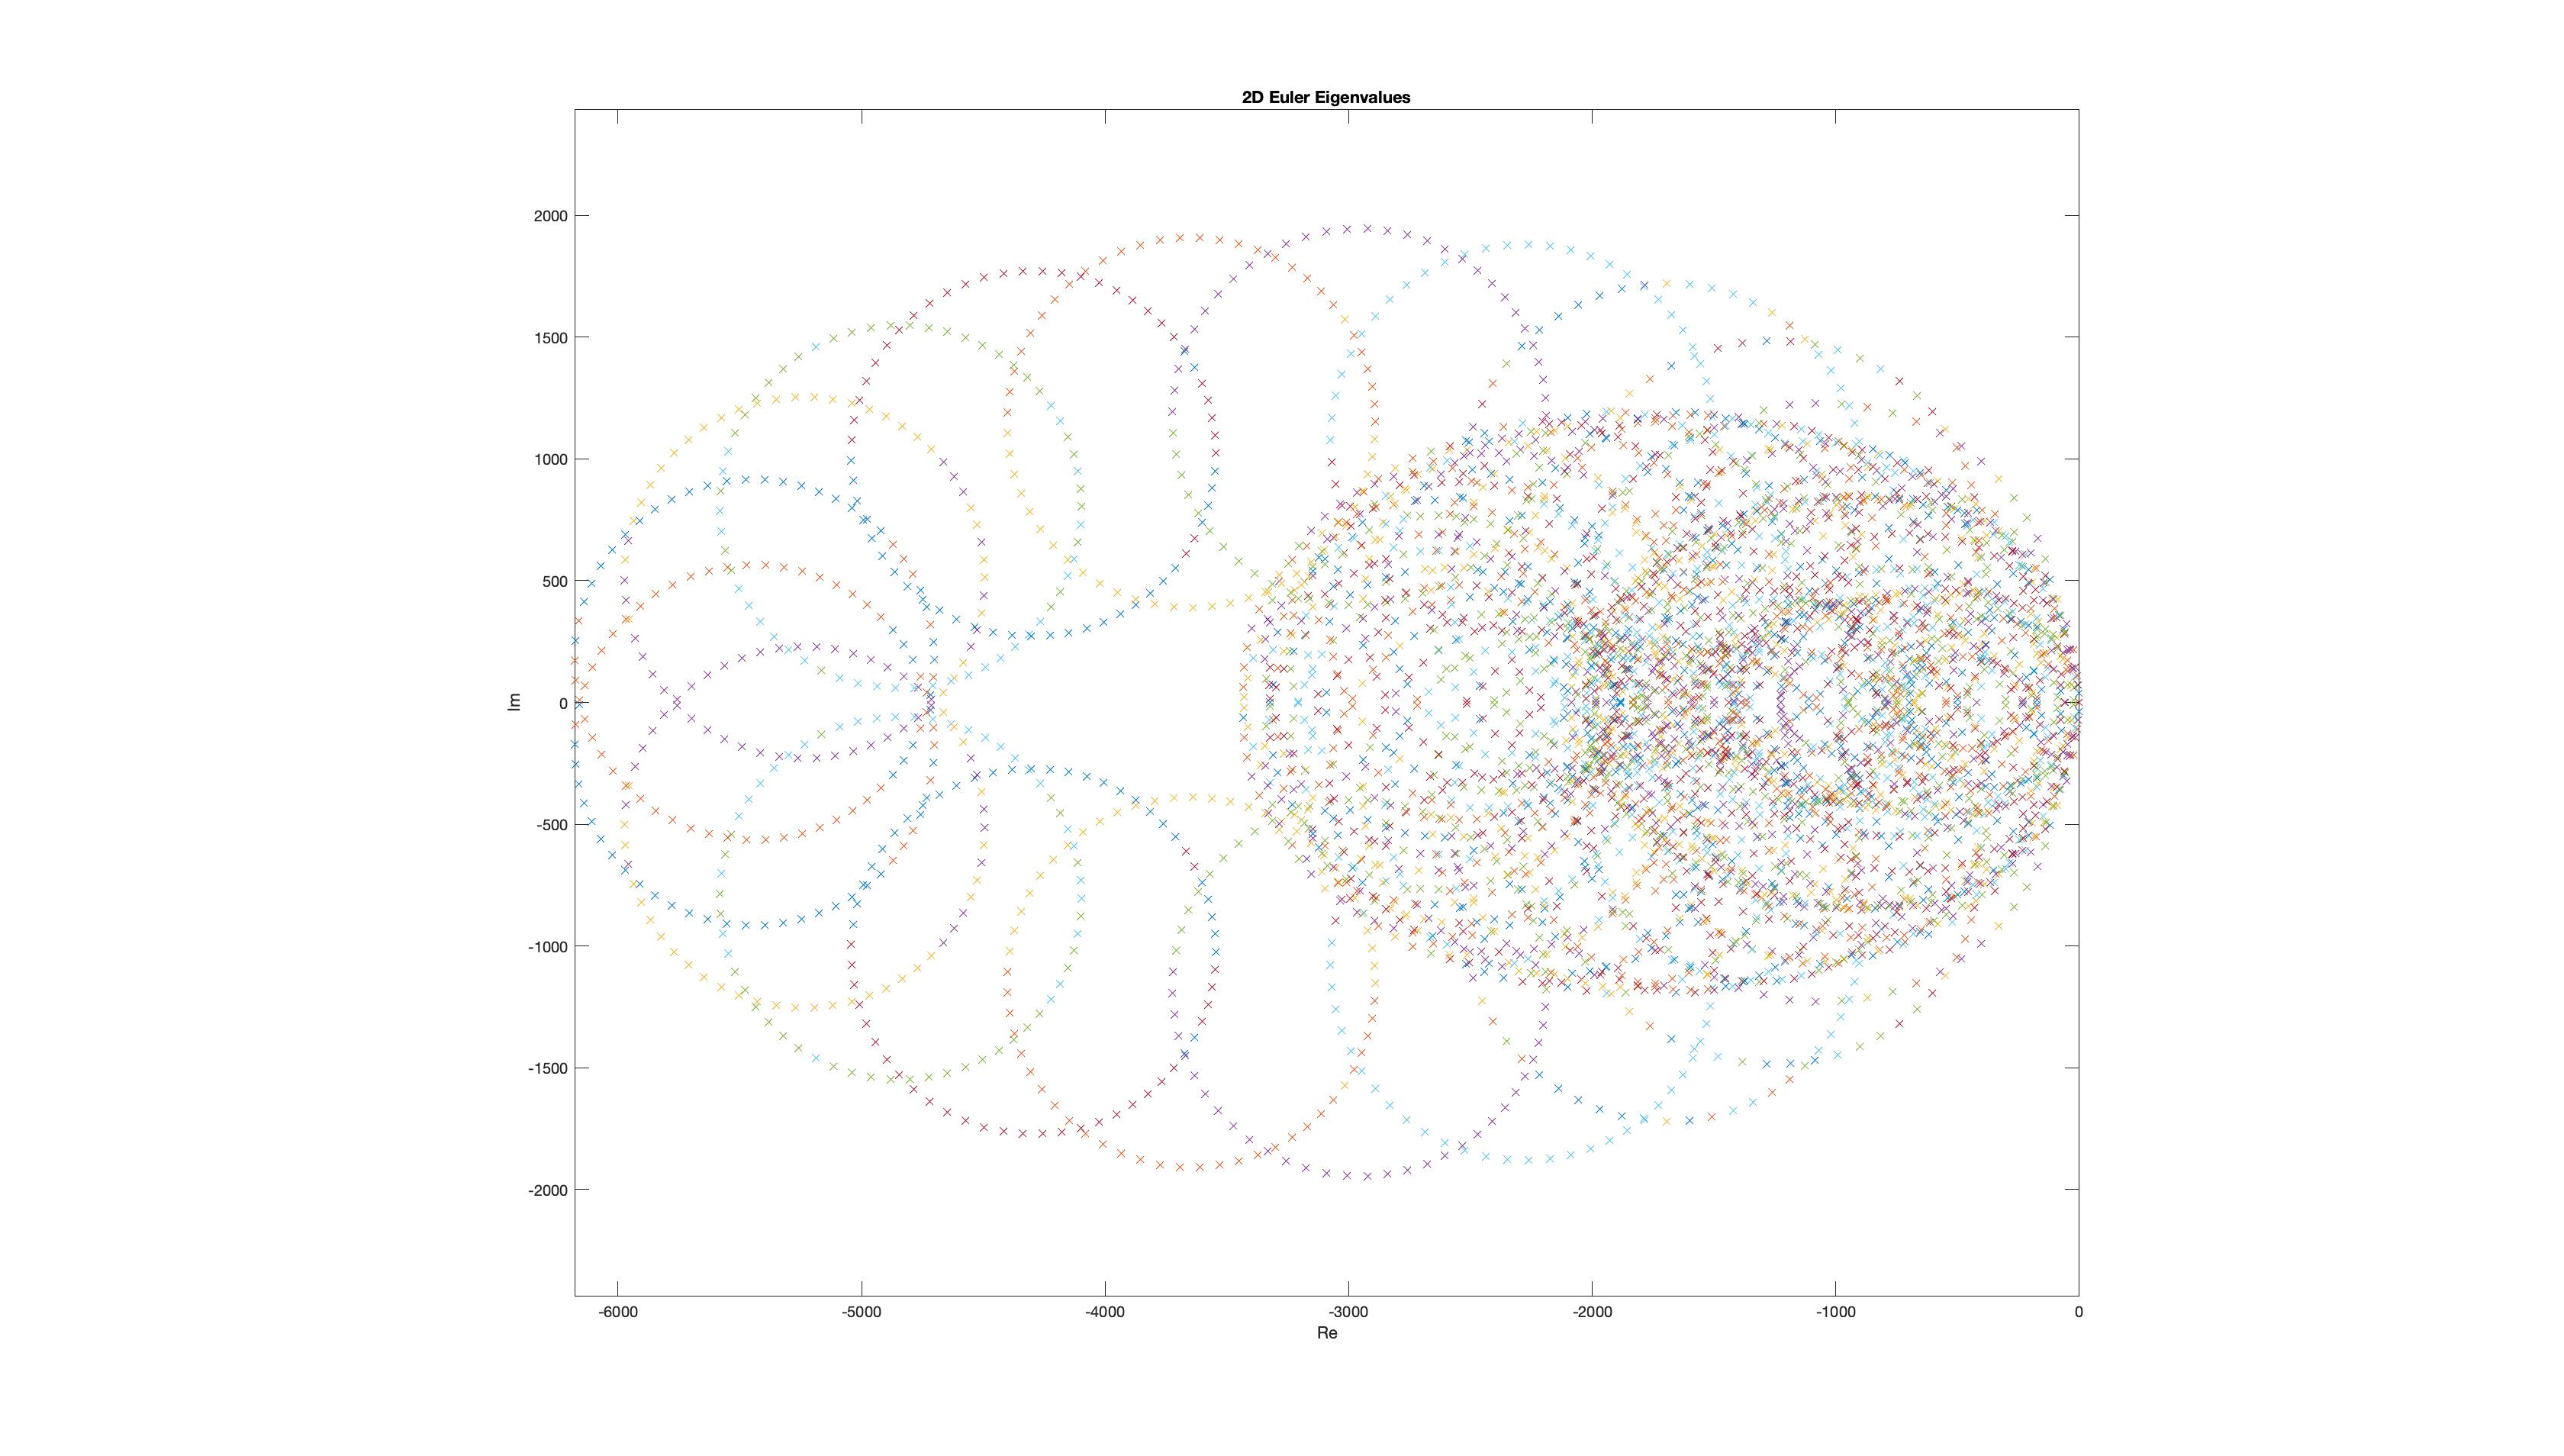
\includegraphics[width=16cm]{2D_euler_eig}
		\centering
	\end{figure}
	
	
	\section{2D Euler Equations with Shock}
	
	INSERT DIAGRAM OF MESH WITH UPSTREAM, DOWNSTREAM AND SHOCK POSITION LABELED.
	
	Here, we will introduce a horizontal oblique shock to the top boundary of the 2D rectangular domain. The governing equations for the 2D Euler conservative variables remain the same, however we will need to solve an evolution equation for the nodes aligned with the shock. All of the nodes will remain fixed except for the nodes that are aligned with the shock which can move slightly up or down in the $y$ direction.
	
	Since the governing equations (\ref{2D_euler}) will be solved on a moving domain, it is convenient to write them in unsteady curvilinear coordinates as follows:
	
	$$ x = f(\xi) $$
	$$ y = g(\eta,\tau) $$
	$$ t = \tau $$
	
	Introducing the Jacobian matrix of the coordinate transformation, $J_{ij} = \frac{\partial x_i}{\partial \xi_j}$ , the Jacobian determinant, $|J|$, and the domain velocity, $x_{i,\tau} = \frac{\partial x_i}{\partial \tau}$ , the governing equations can be written in curvilinear coordinates as
	
	\begin{equation} \label{curvilinear}
		\frac{\partial (|\mathbf{J}| \mathbf{w})}{\partial \tau} + \frac{\partial \tilde{\mathbf{F}_j}}{\partial \xi_j} = 0,
	\end{equation}
	
	where the effective flux $\tilde{\mathbf{F}}$ is defined as
	
	\begin{equation} \label{effective_flux}
		\tilde{\mathbf{F}_i} = |\mathbf{J}| \mathbf{J}_{ij}^{-1}(\mathbf{F}_j - \mathbf{w}x_{j,\tau}).
	\end{equation}
		
	 Equations (\ref{curvilinear}) and (\ref{effective_flux}) account for domain motion in both the $x$ and $y$ directions, however these can be simplified for the case where there is only motion in the $y$ direction.
	 
	 The Jacobian can be simplified to
	 
	 $$
	 \mathbf{\mathbf{J}}_{ij} = \frac{\partial x_i}{\partial \xi_j} = 
	 \begin{bmatrix}
	 	x_\xi & 0 \\
	 	0 & y_\eta
	 \end{bmatrix}
	$$
	
	The Jacobian determinant is now
	
	$$
	|\mathbf{J}| = x_\xi y_\eta
	$$
	 
	 Using the chain rule, the  first term in (\ref{curvilinear}) becomes
	 
	 $$
	 \frac{\partial (|\mathbf{J}| \mathbf{w})}{\partial \tau} = x_\xi \frac{\partial}{\partial \tau} \left( y_\eta \mathbf{w} \right)
	 $$
	 
	 The determinant of the Jacobian multiplied by the inverse of the Jacobian becomes
	 
	 $$
	 |\mathbf{J}| \mathbf{J}_{ij}^{-1} = 
	 \begin{bmatrix}
	 	y_\eta & 0 \\
	 	0 & x_\xi
	 \end{bmatrix}
	 $$
	 
	 The simplified effective fluxes become
	 
	 $$ \tilde{\mathbf{F}_x} = y_\eta \mathbf{F}_x $$
	 
	 $$ \tilde{\mathbf{F}_y}= x_\xi (\mathbf{F}_y - y_\tau \mathbf{w}) $$
	 
	 Substituting these simplifications and effective fluxes into equation (\ref{curvilinear}) yields
	 
	 \begin{equation} \label{moving_domain_equation}
	 	\frac{\partial (|\mathbf{J}| \mathbf{w})}{\partial \tau} + \frac{\partial}{\partial \xi} (y_\eta \mathbf{F}_x) + \frac{\partial}{\partial \eta} (x_\xi (\mathbf{F}_y - y_\tau \mathbf{w})) = 0
	 \end{equation} 
	 
	 \subsection{Non-Shock Layer Nodes}
	 
	 Equation (\ref{moving_domain_equation}) can be further simplified to
	 
	 $$ x_\xi \frac{\partial}{\partial \tau} \left( y_\eta \mathbf{w} \right) + \frac{\partial}{\partial \xi} \tilde{\mathbf{F}_x} + \frac{\partial}{\partial \eta} \tilde{\mathbf{F}_y} = 0 $$
	 
	 $$ x_\xi \frac{\partial}{\partial \tau} \left( y_\eta \mathbf{w} \right) + \frac{\partial}{\partial \xi} (y_\eta \mathbf{F}_x) + \frac{\partial}{\partial \eta} (x_\xi (\mathbf{F}_y - y_\tau \mathbf{w})) = 0$$
	 
	 $$ x_\xi (y_{\eta \tau} \mathbf{w} + y_\eta \mathbf{w}_\tau) + y_\eta \frac{\partial}{\partial \xi} \mathbf{F}_x + x_\xi \left(\frac{\partial}{\partial \eta} \mathbf{F}_y - y_{\eta \tau} \mathbf{w} - y_\tau \mathbf{w}_\eta \right) = 0$$
	 
	 For all of the nodes below the shock layer, $y_{\eta \tau} = 0$
	 
	 $$ x_\xi y_\eta \mathbf{w}_\tau + y_\eta \frac{\partial \mathbf{F}_x}{\partial \xi} + x_\xi \frac{\partial \mathbf{F}_y}{\partial \eta} - x_\xi y_\tau \mathbf{w}_\eta = 0 $$
	 
	 Dividing by the Jacobian $x_\xi y_\eta$ yields
	 
	 $$ \mathbf{w}_\tau + \frac{1}{x_\xi} \frac{\partial \mathbf{F}_x}{\partial \xi} + \frac{1}{y_\eta} \frac{\partial \mathbf{F}_y}{\partial \eta} - y_\tau \frac{1}{y_\eta} \mathbf{w}_\eta = 0 $$
	 
	 The spacial curvilinear coordinates can be converted back to Cartesian coordinates and equation (\ref{curvilinear}) can be written as
	 
	 \begin{equation} \label{curvilinear2}
	 	\mathbf{w}_\tau  - y_\tau \mathbf{w}_y + \frac{\partial \mathbf{F}_x}{\partial x} + \frac{\partial \mathbf{F}_y}{\partial y} = 0
	 \end{equation}
	
	For all the nodes below the shock layer, $y_\tau = 0$. For these nodes, equation (\ref{curvilinear2}) reduces to 
	
	$$ \mathbf{w}_\tau  + \frac{\partial \mathbf{F}_x}{\partial x} + \frac{\partial \mathbf{F}_y}{\partial y} = 0 $$
	
	
	which can be linearized as follows
	
	\begin{equation} \label{curvilinear_interior_linearized}
	\mathbf{w}_\tau  + \frac{\partial \mathbf{F}_x}{\partial \mathbf{w}} \frac{\partial \mathbf{w}}{\partial x}+ \frac{\partial \mathbf{F}_y}{\partial \mathbf{w}} \frac{\partial \mathbf{w}}{\partial y} = 0
	\end{equation}

	Using a small perturbation of $\mathbf{w} = \bar{\mathbf{w}} + \epsilon \mathbf{w}'$, equation (\ref{curvilinear_interior_linearized}) can be Taylor Expanded. Considering only the first order terms of the perturbation yields
	
	$$ \mathbf{w}'_\tau  + \left. \frac{\partial \mathbf{F}_x}{\partial \mathbf{w}} \right|_{\bar{\mathbf{w}}} \frac{\partial \mathbf{w}'}{\partial x} + \left. \frac{\partial \mathbf{F}_y}{\partial \mathbf{w}} \right|_{\bar{\mathbf{w}}} \frac{\partial \mathbf{w}'}{\partial y} = 0 $$
	
	or
	
	\begin{equation} \label{curvilinear_interior_expanded}
		\mathbf{w}'_\tau  + \mathbf{A}_x \frac{\partial \mathbf{w}'}{\partial x} + \mathbf{A}_y \frac{\partial \mathbf{w}'}{\partial y} = 0
	\end{equation}
	
	\subsection{Evolution Equation for Shock Point}
	
	************* INSERT DIAGRAM OF NODE LOCATIONS WITH N, N-1/2 AND N-1. LABEL UPSTREAM, DOWNSTREAM, AND SHOCK LOCATION  *************
	
	Using a small perturbation of $y_N = \bar{y}_N + \epsilon y'$, the Jacobian determinant reduces to
	
	$$ |\mathbf{J}| = x_\xi y_\eta = x_\xi (y_N - y_{N-\frac{1}{2}}) = x_\xi (\bar{y}_N + \epsilon y' - y_{N-\frac{1}{2}}) $$
	
	When $y_\eta = y_N - y_{N-\frac{1}{2}}$.
	
	After considering only the first order terms of the perturbation, the first term of equation (\ref{moving_domain_equation}) becomes
	
	$$ \frac{\partial (|\mathbf{J}| \mathbf{w})}{\partial \tau} = \frac{\partial}{\partial \tau} (x_\xi (\bar{y}_N + \epsilon y' - y_{N-\frac{1}{2}}) (\bar{\mathbf{w}} + \epsilon \mathbf{w}')) = \bar{\mathbf{w}} x_\xi \frac{\partial}{\partial \tau}(y') + x_\xi y_\eta \frac{\partial}{\partial \tau} (\mathbf{w}') $$
	
	***** $\bar{\mathbf{w}} x_\xi \frac{\partial}{\partial \tau}(y')$ IS NOT IN PAPER NOTES AND NOT INCLUDED IN CODE *****
	
	\begin{figure}[h]
		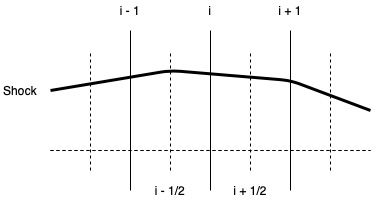
\includegraphics[width=6cm]{shock_point_x}
		\centering
	\end{figure}
	
	The second term of equation (\ref{moving_domain_equation}) can be approximated by taking the difference of the midpoints between the adjacent cells as shown above.
	
	$$ \frac{\partial}{\partial \xi} (y_\eta \mathbf{F}_x) =  (y_\eta \mathbf{F}_x)_{i+\frac{1}{2}} - (y_\eta \mathbf{F}_x)_{i-\frac{1}{2}} $$
	
	Using an upwind flux, $\mathbf{F}_{x,i+\frac{1}{2}}$ can be written as
	
	$$ \mathbf{F}_{x,i+\frac{1}{2}} = \frac{\mathbf{F}_{x,i} + \mathbf{F}_{x,i+1}}{2} - \frac{|\mathbf{A}_x|}{2}(\mathbf{w}_{i+1} - \mathbf{w}_{i})$$
	
	Now using a small perturbation of $\mathbf{w} = \bar{\mathbf{w}} + \epsilon \mathbf{w}'$, 
	
	$$ \mathbf{F}_{x,i+\frac{1}{2}} = \frac{\mathbf{F}_{x,i} + \mathbf{F}_{x,i+1}}{2} - \frac{|\mathbf{A}_x|}{2} (\epsilon \mathbf{w}_{i+1}' - \epsilon \mathbf{w}_i')$$
	
	We can now Taylor expand $\mathbf{F}_{x,i}(\mathbf{w})$ and $\mathbf{F}_{x,i+1}(\mathbf{w})$. Taking the first order terms of $\epsilon$,
	
	$$ \mathbf{F}_{x,i}(\bar{\mathbf{w}} + \epsilon \mathbf{w}') = \mathbf{F}_{x}(\bar{\mathbf{w}}) + A_x \epsilon \mathbf{w}_i' $$
	
	$$ \mathbf{F}_{x,i+1}(\bar{\mathbf{w}} + \epsilon \mathbf{w}') = \mathbf{F}_{x}(\bar{\mathbf{w}}) + A_x \epsilon \mathbf{w}_{i+1}' $$
	
	$y_{\eta,i+\frac{1}{2}}$ can be approximated as the average of $y_{\eta, i}$ and $y_{\eta, i+1}$. Combining this will a small perturbation of $y_N = \bar{y}_N + \epsilon y'$,
	
	$$ y_{\eta,i+\frac{1}{2}} = \bar{y}_N + \epsilon \frac{y_i' + y_{i+1}'}{2} - y_{N-\frac{1}{2}}$$
	
	Now, 
	
	$$ (y_\eta \mathbf{F}_x)_{i+\frac{1}{2}} = \left( \bar{y}_N + \epsilon \frac{y_i' + y_{i+1}'}{2} - y_{N-\frac{1}{2}} \right) \left( \mathbf{F}_{x}(\bar{\mathbf{w}}) + \epsilon \mathbf{A}_x \left( \frac{\mathbf{w}_i' + \mathbf{w}_{i+1}'}{2}\right) - \epsilon \frac{|\mathbf{A}_x|}{2} ( \mathbf{w}_{i+1}' - \mathbf{w}_i') \right) $$
	
	Similarly,
	
	$$ (y_\eta \mathbf{F}_x)_{i-\frac{1}{2}} = \left( \bar{y}_N + \epsilon \frac{y_i' + y_{i-1}'}{2} - y_{N-\frac{1}{2}} \right) \left( \mathbf{F}_{x}(\bar{\mathbf{w}}) + \epsilon \mathbf{A}_x \left( \frac{\mathbf{w}_i' + \mathbf{w}_{i-1}'}{2}\right) - \epsilon \frac{|\mathbf{A}_x|}{2} ( \mathbf{w}_i' - \mathbf{w}_{i-1}') \right) $$
	
	Now subtracting the two equations above yields
	
	\begin{equation}
		\frac{\partial}{\partial \xi} (y_\eta \mathbf{F}_x) = (\bar{y}_N - y_{N-\frac{1}{2}}) \left( \epsilon \mathbf{A}_x \left( \frac{\mathbf{w}_{i+1}' - \mathbf{w}_{i-1}'}{2}\right) - \epsilon \frac{|\mathbf{A}_x|}{2} ( \mathbf{w}_{i+1}' - 2\mathbf{w}_i' + \mathbf{w}_{i-1}') \right) + \epsilon \mathbf{F}_{x}(\bar{\mathbf{w}}) \left( \frac{y_{i+1}' - y_{i-1}'}{2} \right)
	\end{equation}
	
	\begin{figure}[h]
		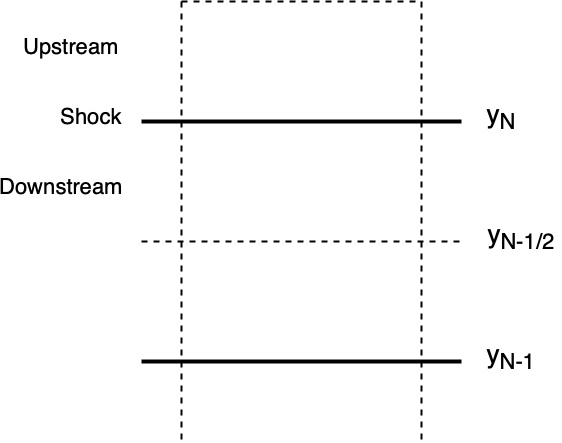
\includegraphics[width=6cm]{shock_point_y}
		\centering
	\end{figure}
	
	The third term of equation (\ref{moving_domain_equation}) can be approximated by taking the difference of the top cell and the midpoint of the cell below.
	
	$$ \frac{\partial}{\partial \eta} (x_\xi (\mathbf{F}_y - y_\tau \mathbf{w})) =  (x_\xi (\mathbf{F}_y - y_\tau \mathbf{w}))_{N} - (x_\xi (\mathbf{F}_y - y_\tau \mathbf{w}))_{N-\frac{1}{2}} $$
	
	Since here we are using a half cell, 
	
	$$ x_{\xi,N} = x_{\xi, N-\frac{1}{2}} = \frac{\Delta x}{2} $$
	
	*************** SHOULD THIS BE $\Delta x$? ***********
	
	Using a small perturbation of $y_N = \bar{y}_N + \epsilon y'$ and equation (\ref{}), 
	
	$$ y_{\tau,N} = \bar{y}_{\tau,N} + \epsilon y'_{\tau,N} = \epsilon y'_{\tau,N} = - \epsilon \mathbf{u}_u \frac{1}{\Delta x} \left( \frac{\partial y'}{\partial \xi} \right)_N $$
	
	Since $\mathbf{F}_{y,N}$ lies directly on a mesh node,
	
	$$ \mathbf{F}_{y,N} = \mathbf{F}_{y}(\bar{\mathbf{w}}_N) $$
	
	Now using a small perturbation of $\mathbf{w} = \bar{\mathbf{w}} + \epsilon \mathbf{w}'$,
	
	% THIS EQUATION USES A CENTRAL DIFFFERENCE FOR Y
	
	% $$ (x_\xi (\mathbf{F}_y - y_\tau \mathbf{w}))_{N} = \frac{\Delta x}{2} \left( \mathbf{F}_{y}(\bar{\mathbf{w}}) + \epsilon \mathbf{u}_u \frac{1}{\Delta x} \left( \frac{y'_{i+1} - y'_{i-1}}{2 \Delta x} \right) (\bar{\mathbf{w}}_N + \epsilon \mathbf{w}'_N) \right) $$
	
	\begin{equation} \label{shock_term2_pt1}
		(x_\xi (\mathbf{F}_y - y_\tau \mathbf{w}))_{N} = \frac{\Delta x}{2} \left( \mathbf{F}_{y}(\bar{\mathbf{w}}_N) + \epsilon \mathbf{u}_u \frac{1}{\Delta x} \left( \frac{\partial y'}{\partial \xi} \right)_N (\bar{\mathbf{w}}_N + \epsilon \mathbf{w}'_N) \right)
	\end{equation}
	
	
	Using an upwind flux, $\mathbf{F}_{y,N-\frac{1}{2}}$ can be written as
	
	$$ \mathbf{F}_{y,N-\frac{1}{2}} = \frac{\mathbf{F}_{y,N} + \mathbf{F}_{y,N-1}}{2} - \frac{|\mathbf{A}_y|}{2}(\mathbf{w}_{N} - \mathbf{w}_{N-1})$$
	
	Now using a small perturbation of $\mathbf{w} = \bar{\mathbf{w}} + \epsilon \mathbf{w}'$, 
	
	$$ \mathbf{F}_{y,N-\frac{1}{2}} = \frac{\mathbf{F}_{y,N} + \mathbf{F}_{y,N-1}}{2} - \frac{|\mathbf{A}_y|}{2} (\epsilon \mathbf{w}_{N}' - \epsilon \mathbf{w}_{N-1}')$$
	
	We can now Taylor expand $\mathbf{F}_{y,N}(\mathbf{w})$ and $\mathbf{F}_{y,N-1}(\mathbf{w})$. Taking the first order terms of $\epsilon$,
	
	$$ \mathbf{F}_{y,N}(\bar{\mathbf{w}} + \epsilon \mathbf{w}') = \mathbf{F}_{y}(\bar{\mathbf{w}}) + A_y \epsilon \mathbf{w}_N' $$
	
	$$ \mathbf{F}_{y,N-1}(\bar{\mathbf{w}} + \epsilon \mathbf{w}') = \mathbf{F}_{y}(\bar{\mathbf{w}}) + A_y \epsilon \mathbf{w}_{N-1}' $$
	
	Since only the top layer of the mesh is allowed to move, $y_{\tau,N-\frac{1}{2}}=0$
	
	Now,
	
	\begin{equation} \label{shock_term2_pt2}
		(x_\xi (\mathbf{F}_y - y_\tau \mathbf{w}))_{N-\frac{1}{2}} = \frac{\Delta x}{2} \left( \mathbf{F}_{y}(\bar{\mathbf{w}}) + \epsilon \mathbf{A}_y \left( \frac{\mathbf{w}_N' + \mathbf{w}_{N-1}'}{2}\right) - \epsilon \frac{|\mathbf{A}_y|}{2} ( \mathbf{w}_N' - \mathbf{w}_{N-1}') \right)
	\end{equation}
	
	Now subtracting  equations (\ref{shock_term2_pt1}) and (\ref{shock_term2_pt2}) and taking only the first order terms of $\epsilon$ yields
	
	\begin{equation}
		\frac{\partial}{\partial \eta} (x_\xi (\mathbf{F}_y - y_\tau \mathbf{w})) = \epsilon \frac{\mathbf{u}_u \bar{\mathbf{w}}}{2} \left( \frac{\partial y'}{\partial \xi} \right)_N - \epsilon \frac{\mathbf{A}_y \Delta x}{2} \left( \frac{\mathbf{w}_N' + \mathbf{w}_{N-1}'}{2} \right) + \epsilon \frac{|\mathbf{A}_y| \Delta x}{4} ( \mathbf{w}_N' - \mathbf{w}_{N-1}')
	\end{equation}
	
	
	
	

\end{document}